\documentclass[onecolumn,notitlepage,superscriptaddress, amsmath,amssymb,longbibliographyaps,floatfix]{revtex4-1}


\usepackage{amssymb}
\usepackage{amsthm}
\usepackage{amsmath}
\usepackage{natbib}
\usepackage{bm}
\usepackage{tikz}
\usepackage{pgfplots,tikz-3dplot}
\usepackage{ar}

\newcommand{\aver}[1]{ \! \left\langle {#1} \right \rangle \!}




\begin{document}
\title{Evolution of the 2D wake with AR and Re}
\author{}
\date{\today}
\maketitle



\begin{figure}
  \centering
  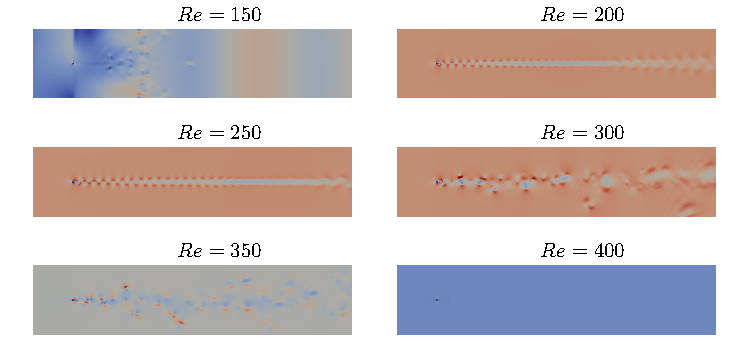
\includegraphics[width=\textwidth]{./fig/AR1.pdf}
  \caption{$\mathcal{AR}=1$.}
  \label{fig:AR1}
\end{figure}

\begin{figure}
  \centering
  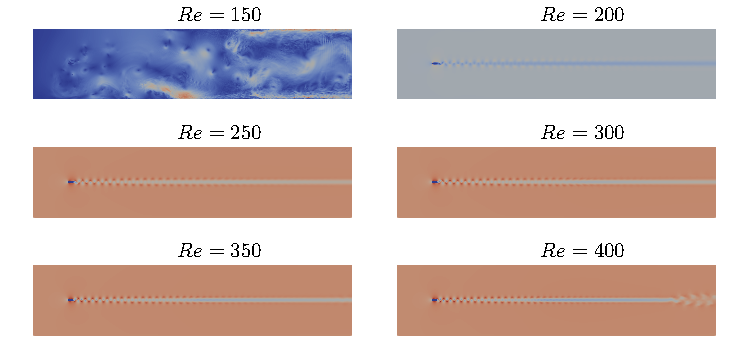
\includegraphics[width=\textwidth]{./fig/AR3.pdf}
  \caption{$\mathcal{AR}=3$.}
  \label{fig:AR3}
\end{figure}

\begin{figure}
  \centering
  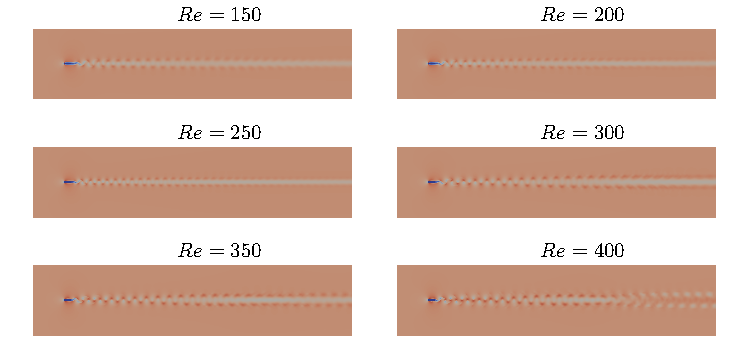
\includegraphics[width=\textwidth]{./fig/AR4p5.pdf}
  \caption{$\mathcal{AR}=4.5$.}
  \label{fig:AR4p5}
\end{figure}

\begin{figure}
  \centering
  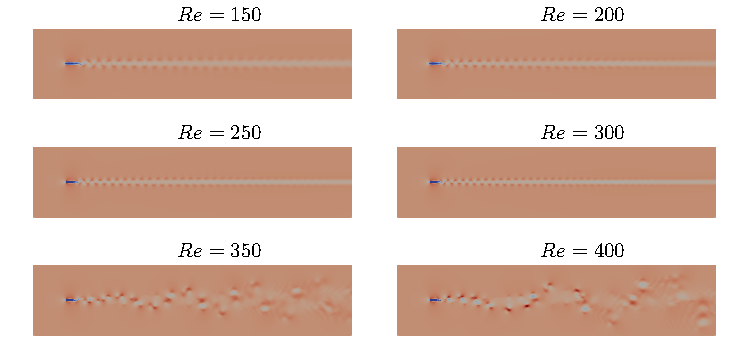
\includegraphics[width=\textwidth]{./fig/AR5.pdf}
  \caption{$\mathcal{AR}=5$.}
  \label{fig:AR5}
\end{figure}

\begin{figure}
  \centering
  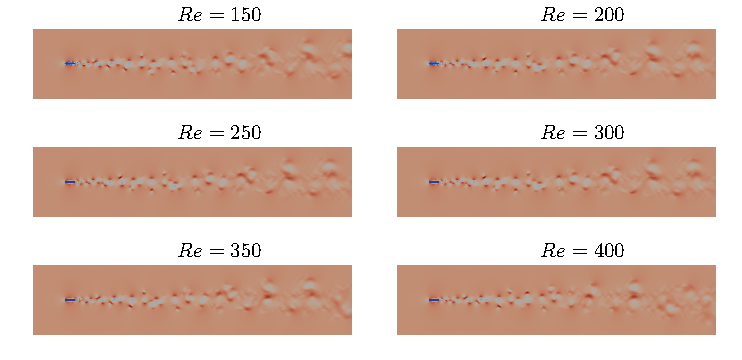
\includegraphics[width=\textwidth]{./fig/AR7.pdf}
  \caption{$\mathcal{AR}=7$.}
  \label{fig:AR7}
\end{figure}

\bibliographystyle{jfm}     % mathematics and physical sciences

\bibliography{../Wallturbulence}
	
	
\end{document}



